\documentclass[11pt,a4paper,oneside]{book}
% default
\usepackage[hmargin={1.25in,1.25in},vmargin={1.25in,1.25in}]{geometry}
% draft
%\usepackage[hmargin={1in,1in},vmargin={1in,1in}]{geometry}

\usepackage[OT1]{fontenc}
\usepackage{fontspec}
\usepackage[Greek]{ucharclasses}

\newfontfamily{\greekfont}[Scale=MatchLowercase]{cmunrm.otf}
%\setTransitionsForGreek{\begingroup\greekfont}{\endgroup}

\makeindex
\usepackage{textcomp}
\usepackage{fancyhdr}
\usepackage{makeidx}
\pagestyle{myheadings}
\fancyhf{}
\rhead[\leftmark]{thepage}

\usepackage{url}

\parindent0em
\parskip1.5ex

%%

%%%% Packages
\usepackage{acronym}
\usepackage{amsmath}
\usepackage{amsthm}
\usepackage{amsfonts}
\usepackage{amssymb}
\usepackage{xspace}
\usepackage{enumitem}
\usepackage{mathrsfs}

%%%% PGF/TikZ
\usepackage{tikz}
\usetikzlibrary{arrows,decorations,backgrounds,positioning,fit,petri}
\tikzset{
	x=0.16\linewidth,
	y=0.16\linewidth,
	>=stealth',
	bend angle=30,
	every place/.style={
		draw=black,
		minimum size=0.055\linewidth
	},
	every transition/.style={
		fill=black,
		minimum height=0.055\linewidth,
		inner xsep=0pt,
		minimum width=3pt
	}
}

%%%% Theorems
\theoremstyle{plain}
%\newtheorem{lemme}{Lemme}
%\newtheorem{prop}{Proposition}
\theoremstyle{definition}
\newtheorem{defi}{Definition}
%\theoremstyle{remark}
%\newtheorem{conv}{Convention}

%%%% Matrices
\makeatletter
\newif\if@borderstar
\def\bordermatrix{\@ifnextchar*{%
\@borderstartrue\@bordermatrix@i}{\@borderstarfalse\@bordermatrix@i*}%
}
\def\@bordermatrix@i*{\@ifnextchar[{\@bordermatrix@ii}{\@bordermatrix@ii[()]}}
\def\@bordermatrix@ii[#1]#2{%
\begingroup
\m@th\@tempdima8.75\p@\setbox\z@\vbox{%
\def\cr{\crcr\noalign{\kern 2\p@\global\let\cr\endline }}%
\ialign {$##$\hfil\kern 2\p@\kern\@tempdima & \thinspace %
\hfil $##$\hfil && \quad\hfil $##$\hfil\crcr\omit\strut %
\hfil\crcr\noalign{\kern -\baselineskip}#2\crcr\omit %
\strut\cr}}%
\setbox\tw@\vbox{\unvcopy\z@\global\setbox\@ne\lastbox}%
\setbox\tw@\hbox{\unhbox\@ne\unskip\global\setbox\@ne\lastbox}%
\setbox\tw@\hbox{%
$\kern\wd\@ne\kern -\@tempdima\left\@firstoftwo#1%
\if@borderstar\kern2pt\else\kern -\wd\@ne\fi%
\global\setbox\@ne\vbox{\box\@ne\if@borderstar\else\kern 2\p@\fi}%
\vcenter{\if@borderstar\else\kern -\ht\@ne\fi%
\unvbox\z@\kern-\if@borderstar2\fi\baselineskip}%
\if@borderstar\kern-2\@tempdima\kern2\p@\else\,\fi\right\@secondoftwo#1 $%
}\null \;\vbox{\kern\ht\@ne\box\tw@}%
\endgroup
}
\makeatother


%%%% Document specific
\newcommand{\tupleN}{\ensuremath{\mathcal{N}}\xspace}
\newcommand{\tupleS}{\ensuremath{\mathcal{S}}\xspace}
\newcommand{\marq}{\ensuremath{\mathbf{m}}\xspace}
\newcommand{\marqi}{\ensuremath{\mathbf{m}_0}\xspace}
\newcommand{\marqp}{\ensuremath{\mathbf{m'}}\xspace}
\newcommand{\marqpi}{\ensuremath{\mathbf{m'}_0}\xspace}
\newcommand{\PT}{\ensuremath{\langle P,T\rangle}\xspace}
\newcommand{\PTm}{\ensuremath{\langle P,T, \marqi\rangle}\xspace}
\newcommand{\PTP}{\ensuremath{\langle P,T,\mathbb{P}\rangle}\xspace}
\newcommand{\PTPm}{\ensuremath{\langle P,T,\mathbb{P}, \marqi\rangle}\xspace}
\newcommand{\NPT}{\ensuremath{\tupleN = \PT}\xspace}
\newcommand{\NPTm}{\ensuremath{\tupleN = \PTm}\xspace}
\newcommand{\SPTP}{\ensuremath{\tupleS = \PTP}\xspace}
\newcommand{\SPTPm}{\ensuremath{\tupleS = \PTPm}\xspace}
\newcommand{\fire}[1]{\stackrel{#1}{\to}}
\newcommand{\firev}[1]{\stackrel{#1}{\to}_v}
\newcommand{\matI}{\mathbf{I}}
\newcommand{\matO}{\mathbf{O}}
\newcommand{\matIN}{\matI_\tupleN}
\newcommand{\matON}{\matO_\tupleN}
\newcommand{\matIS}{\matI_\tupleS}
\newcommand{\matOS}{\matO_\tupleS}
\newcommand{\Ecov}{\ensuremath{\mathscr{E}\text{-cov}}\xspace}
\newcommand{\Ucov}{\ensuremath{\mathscr{U}\text{-cov}}\xspace}
% prec pleq npleq
\newcommand{\pleq}{\preccurlyeq}
\newcommand{\npleq}{\npreccurlyeq}

%%%% Layout
\setlist[itemize]{noitemsep,nolistsep}
%\makeatletter
%\parindent 10pt
%\topsep 4pt plus 1pt minus 2pt
%\partopsep 1pt plus 0.5pt minus 0.5pt
%\itemsep 2pt plus 1pt minus 0.5pt
%\parsep 2pt plus 1pt minus 0.5pt
%
%\leftmargin 10pt \leftmargini\leftmargin \leftmarginii 10pt
%\leftmarginiii 5pt \leftmarginiv 5pt \leftmarginv 5pt \leftmarginvi 5pt
%\labelwidth\leftmargini\advance\labelwidth-\labelsep \labelsep 5pt
%
%\def\@listi{\leftmargin\leftmargini}
%\def\@listii{\leftmargin\leftmarginii
%   \labelwidth\leftmarginii\advance\labelwidth-\labelsep
%   \topsep 2pt plus 1pt minus 0.5pt
%   \parsep 1pt plus 0.5pt minus 0.5pt
%   \itemsep \parsep}
%\def\@listiii{\leftmargin\leftmarginiii
%    \labelwidth\leftmarginiii\advance\labelwidth-\labelsep
%    \topsep 1pt plus 0.5pt minus 0.5pt
%    \parsep \z@ \partopsep 0.5pt plus 0pt minus 0.5pt
%    \itemsep \topsep}
%\def\@listiv{\leftmargin\leftmarginiv
%     \labelwidth\leftmarginiv\advance\labelwidth-\labelsep}
%\def\@listv{\leftmargin\leftmarginv
%     \labelwidth\leftmarginv\advance\labelwidth-\labelsep}
%\def\@listvi{\leftmargin\leftmarginvi
%     \labelwidth\leftmarginvi\advance\labelwidth-\labelsep}
%
%\abovedisplayskip 7pt plus2pt minus5pt%
%\belowdisplayskip \abovedisplayskip
%\abovedisplayshortskip  0pt plus3pt%
%\belowdisplayshortskip  4pt plus3pt minus3pt%
%\makeatother


%%%% TMP
\newcommand{\todo}[1]{[TODO: #1]}


\begin{document}

\frontmatter
\begin{titlepage}
\begin{center}
\textbf{UNIVERSIT\'E LIBRE DE BRUXELLES}\\
\textbf{Faculté des Sciences}\\
\textbf{Département d'Informatique}
\vfill{}\vfill{}

{\Huge  The Coverability problem \vspace*{.5cm}  \linebreak[4] for parametric Petri nets}

{\Huge \par}
\begin{center}{\LARGE Alexis Reynouard}\end{center}{\Huge \par}
\vfill{}\vfill{}
\begin{flushright}{\large \textbf{Promotor :} Prof. Gilles Geeraerts}\hfill{}{\large Master Thesis in Computer Sciences}\\
{\large }\hfill{}{}\end{flushright}{\large\par}
\vfill{}\vfill{}\enlargethispage{3cm}
\textbf{Academic year 2018~-~2019}
\end{center}
\end{titlepage}
\newpage
\thispagestyle{empty} 
\null

\newenvironment{vcenterpage}
{\newpage\thispagestyle{empty} 
\vspace*{\fill}}
{\vspace*{\fill}\par\pagebreak}

%\begin{vcenterpage}
%\begin{flushright}
%    \large\em\null\vskip1in 
%    You may want\\
%   to write a dedication here\vfill
%  \end{flushright}
%\end{vcenterpage}
%\thispagestyle{empty}
%\vspace*{5cm}
%
%\begin{quotation}
%\noindent ``\emph{You may also include one or more general quotes related to your topic.}''
%\begin{flushright}\textbf{Name of the author, date}\end{flushright}
%\end{quotation}
%
%\medskip
%
%\begin{quotation}
%\noindent ``\emph{Another quote.}''
%\begin{flushright}\textbf{Name of the author, date}\end{flushright}
%\end{quotation}
%\chapter*{Acknowledgment}
%\thispagestyle{empty} 
%
%\noindent I want to thank ...

\thispagestyle{empty} 
\setcounter{page}{0}
\tableofcontents

\acrodef{PN}{Petri net}
\acrodef{PPN}{parametric Petri net}

\mainmatter
\setcounter{page}{1}

\chapter{Introduction}
\acp{PN} are a mathematical and graphical model introduced by Carl Adam Petri in 1962 \citep{Petri62,Petri66}.
It was successfully used to analyse systems in a wide range of domains, and has proven to be particularly successful for the formal verification of asynchronous systems.

In their standard definition, \acp{PN} are instantiated through many natural numbers\footnote{\lang{i.e.} a \ac{PN} may be represented as a pair of matrices whose the values are from $\naturals$.} which may represent, for example, the amount of resource needed for a given action to be carried out.

The introduction of parameters into the model to avoid the need to state these values explicitly%
\footnote{One can find in the literature many other way to use parameters in \acp{PN}. For example, place and~/~or transitions may also be parameters in order to dynamically change the network structure, like in \cite{Christensen97}.}
may have several benefits:
it may allow performing analysis of a whole family of \acp{PN} efficiently, like in \cite{Abdulla13}, or to model dynamic changes in the system, as introduced by \cite{Badouel99} as a subclass of reconfigurable nets.

The use of parameters increases the modelling power of \acp{PN} but also make some basic coverability problems undecidable in the general case \cite{David17}.

We adopt the parametric Petri net model introduced by \cite{David17}, which seems the most general, and we study the existing results and algorithms for plain Petri nets to find out whether they still hold or how to adapt them to the parametric model.

The rest of the document is as follows:
In this first part, we define the plain Petri net model (\lang{i.e.} the classical one) and the parametric model.
We then briefly motivate our study, \todo{give concrete examples of applications,} and give an overview of the previous works on parametrisation of \acp{PN}.
Finally, we place the \ac{PN} model in a broader model family: the \acp{WSTS}.\\
In a second part, we recall, first, the classical results that we will study on this new model, second, the results already obtained for the parametrized Petri net model as we have defined them.\\
Then, we focus on the parametric Petri net model to establish whether the results related to the coverability problem in the plain Petri net model still hold or if the algorithms may be adapted to this new model.

\acresetall

\section{Definitions}
\begin{defi}[\acl{PN}]
  A \acf{PN} \tupleN is a weighted oriented bipartite graph, whose the two subsets of vertices define a tuple \PT where:
  \begin{itemize}
    \item $P$ is a finite set of places,
    \item $T$ is a finite set of transitions.
  \end{itemize}
  For each transition $t \in T$ are defined (exactly) these two functions:
  \begin{itemize}
    \item $I_t : P \mapsto \mathbb{N}$ associates to each place the weight of the edge to $t$ \emph{(input weight)},
    \item $O_t : P \mapsto \mathbb{N}$ associates to each place the weight of the edge from $t$ \emph{(output weight)}.
  \end{itemize}
  It is denoted by $t = \langle I_t, O_t \rangle$.
  Because these functions define the edges of the graph, a \ac{PN} is completely defined by the tuple \PT and so is denoted by \NPT.
\end{defi}

\begin{defi}[marking]
  Given a set of place $P$, a marking over $P$ is a function $\marq : P \mapsto \mathbb{N}$ that associates $\marq(p)$ tokens to each place $p \in P$.
\end{defi}

An order on the markings is essential for the analysis of \acp{PN}. The order we will define is a well quasi order and a partial order.

\begin{defi}[quasi order]
  A quasi order on a set $\mathcal{E}$ is a binary relation $R$ that is:
  \begin{align*}
    \text{reflexive: } &&\forall x \in \mathcal{E},\ & x \mathrel{R} x \\
    \text{transitive: } &&\forall (x, y, z) \in \mathcal{E}^3,\ & (x \mathrel{R} y\land y \mathrel{R} z)\Rightarrow x \mathrel{R} z
  \end{align*}
\end{defi}

\begin{defi}[well quasi order]
  A well quasi order $\sqsubseteq$ on a set $\mathcal{E}$ is a quasi order on $\mathcal{E}$ such that, for any infinite sequence $s = e_0, e_1, e_2, \dots$ of elements from $\mathcal{E}$, there exist indices $i < j$ with $e_i \sqsubseteq e_j$. That is, there is no infinite antichain in $\mathcal{E}$ for this relation.
\end{defi}

\begin{defi}[partial order]
  A partial order on a set $\mathcal{E}$ is a quasi order $R$ that is
  \begin{align*}
    \text{antisymmetric: } &&\forall (x, y) \in \mathcal{E}^2,\ & (x \mathrel{R} y\land y \mathrel{R} x)\Rightarrow x = y
  \end{align*}
\end{defi}

\begin{defi}[partial order \(\pleq\) on the markings]
  Given a set of places $P$, the partial order \(\pleq \subseteq \mathbb{N}^{|P|} \times \mathbb{N}^{|P|}\) is such that for all pair of markings \((\marq_1, \marq_2) \in \mathbb{N}^{|P|} \times \mathbb{N}^{|P|}\) we have that \(\marq_1 \pleq \marq_2\) if and only if for all place \(p \in P : \marq_1(p) \leq \marq_2(p)\).
\end{defi}

\(\marq \prec \marqp\) denote that \(\marq \pleq \marqp \text{ and } \marqp \npleq \marq\).

\begin{lemm}[\cite{Dickson13}]
  \label{lemm:wqo}
  $\pleq$ is a well quasi order.
\end{lemm}

The following result will be useful in the sequel.

\begin{lemm}[\cite{Brams83}]
  The \ac{PN} model is \emph{strongly monotonic with regard to $\pleq$}. That is, for all \ac{PN} $\tupleN = \PTm$, for all transition $t \in T$ and for all markings $\marq_1, \marq_2, \marq_3$ of \tupleN such that $\marq_1 \prec \marq_2$ and $\marq_1 \fire{t} \marq_3$, there exists a marking $\marq_4$ of \tupleN such that $\marq_2 \fire{t} \marq_4$ and $\marq_3 \prec \marq_4$. 
\end{lemm}

In this work we will focus on an extension of the \ac{PN} model, the \ac{PPN} model, that is extended thanks to the use of parameters as input and output weights.

\begin{defi}[\acl{PPN}]
  A \acf{PPN} \SPTP is a weighted oriented bipartite graph with a finite set $\mathbb{P}$ of parameters. The two subsets of vertices are:
  \begin{itemize}
    \item $P$: a finite set of places,
    \item $T$: a finite set of transitions,
  \end{itemize}
  For each transition $t \in T$ are defined the following functions:
  \begin{itemize}
    \item $I_t : P \mapsto \mathbb{N} \cup \mathbb{P}$ associates to each place the weight of the edge to $t$ \emph{(input weight)},
    \item $O_t : P \mapsto \mathbb{N} \cup \mathbb{P}$ associates to each place the weight of the edge from $t$ \emph{(output weight)}.
  \end{itemize}
\end{defi}

As for plain \acp{PN}, this is denoted $t = \langle I_t, O_t \rangle$.

\begin{defi}[parametric marking]
  Given a set of place $P$, a parametric marking over $P$ is a function $\marq : P \mapsto \mathbb{N} \cup \mathbb{P} $ that associates $\marq(p)$ tokens to each place $p \in P$.
\end{defi}

A marking of a \ac{PN} \NPT is a marking over $P$.
A marking of a \ac{PPN} \SPTP is a \emph{parametric} marking over $P$.
Note that a marking \marq is a parametric marking where $\marq(p) \in \mathbb{N}$ for all $p \in P$.

\begin{defi}[initialized (parametric) \ac{PN}]
  An initialized \ac{PN} \NPTm (resp. \ac{PPN} \SPTPm) is a \ac{PN} (resp. \ac{PPN}) with an initial marking \marqi.
\end{defi}

This is sometimes called a \emph{marked (parametric) \ac{PN}}.
We will often refer to an initialized (parametric) \ac{PN} loosely as a (parametric) \ac{PN}.

The figure~\ref{fig:parametric-petri-net-example} shows an example of \ac{PPN} whose $\mathbb{P} = \{a, b\}$ and with an initial marking \marqi such that $\marqi(p_1) = 1$, $\marqi(p_2) = a$ and $\marqi(p_3) = 0$. The circles represent the places, the rectangles are the transitions and the dots are the tokens. If the number of token at a given place is parametric (\lang{i.e.} depends on a parameter of $\mathbb{P}$), it is written inside the circle. An arrow from a place $p$ and to a transition $t$ denotes that $I_t(p) = 1$. If there is no arrow from $p$ to $t$, $I_t(p) = 0$. If $I_t(p) \notin \{0, 1\}$, a label with the value of $I_t(p)$ is added to the arrow.
Symmetrically, the arrows from the transitions to the places indicate the output weights.

\begin{figure}[h]
  \centering
  \center
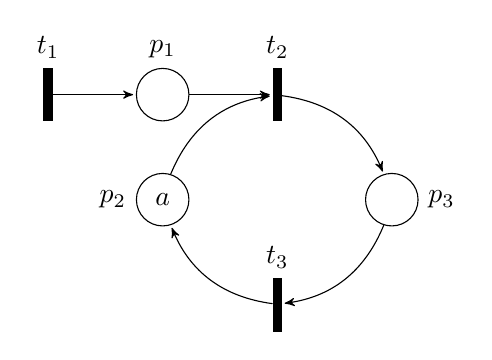
\begin{tikzpicture}[auto,x=0.12\linewidth,y=0.11\linewidth]
	\node [place] (d) [label=$p_1$] at (4,2) {};
	\node [place] (l) [label=west:$p_2$] at (4,1) {$a$};
	\node [place] (o) [label=east:$p_3$] at (6,1) {};
	
	\node [transition] (S) [label=$t_1$] at (3,2) {}
	edge [post] (d);
	\node [transition] (C) [label=$t_2$] at (5,2) {}
	edge [pre]  (d)
	edge [pre,  bend right] (l)
	edge [post, bend left]  (o);
	\node [transition] (F) [label=$t_3$] at (5,0) {}
	edge [pre,  bend right] (o)
	edge [post, bend left]  (l);
\end{tikzpicture}
\par

  \par
  \caption{An initialized \ac{PPN}}
  \label{fig:parametric-petri-net-example}
\end{figure}

We usually set an order on the places.
This allows to view the markings as vectors (here, \marqi is the column vector $(1, a, 0)^T$, where $\cdot^T$ is the transpose operator) as well as the $I$ and $O$ functions.
Likewise, we define an order on the transitions.
Therefore, $I_t$ and $O_t$ denote respectively the $I$ and $O$ functions defined for the $t$\textsuperscript{th} transition (here, $I_1 = (0, 0, 0)^T$ and $O_1 = (b, 0, 0)^T$).
Given a \ac{PPN} \SPTP, the backward and forward incidence matrices $\matIS \in (\mathbb{N} \cup \mathbb{P})^{|P|\times|T|}$ and $\matOS \in (\mathbb{N} \cup \mathbb{P})^{|P|\times|T|}$ are naturally defined by $\matIS(p, t) = I_t(p)$ and $\matOS(p, t) = O_t(p)$.
($\tupleS$ is omitted when it is obvious from the context.)
%In addition, it makes the equivalence between \acp{PN} and \emph{vector addition systems} introduced in \cite{Karp69} more explicit and
This allows to use linear algebra to analyse \acp{PN}.

\begin{figure}[h]
	\[
		\matI = \bordermatrix[{[]}]{%
					& t_1 & t_2 & t_3 \cr
			p_1 & 0   & 1   & 0   \cr
			p_2 & 0   & 1   & 0   \cr
			p_3 & 0   & 0   & 1   }
		\mspace{56mu}
		\matO = \bordermatrix[{[]}]{%
					& t_1 & t_2 & t_3 \cr
			p_1 & b   & 0   & 0   \cr
			p_2 & 0   & 0   & 1   \cr
			p_3 & 0   & 1   & 0   }
	\]
  \caption{The incidence matrices of the \ac{PN} from figure \ref{fig:parametric-petri-net-example}}
  \label{fig:incidence-matrices-example}
\end{figure}

%\begin{defi}[Vector addition system]
%  A vector addition system of dimension $n$ is a pair $\langle d, W\rangle$ where $d \in \mathbb{N}^n$ is called the \emph{start vector} and $W$ is a finite set of vector $\mathbb{Z}^n$.
%\end{defi}
%This corresponds to the definition of an initialized \ac{PN} and \todo{we will see that the semantic corresponds too}.

\subsection{Operational semantic of \acp{PN}}

Given a \ac{PN} \NPT and a marking \marq on \tupleN, a transition $t \in T$ is said \emph{enabled} by \marq if $\forall p \in P : \marq(p) \geq I_t(p)$. An enabled transition can be \emph{fired} to produce a new marking \marqp such that $\forall p \in P : \marqp(p) = \marq(p) - I_t(p) + O_t(p)$. This is denoted by $\marq \fire{t} \marqp$.
It is important to note that the effect of a transition is to add or remove a constant number of tokens at each place and does not depend on the marking from which it is fired. A \ac{PN} transition is said to have a \emph{constant effect}.
\todo{Note difference when talking about {\textomega}-Petri nets}

Here are some additional notations:
\begin{itemize}
  \item $\marq \rightarrow \marqp$ denotes that there exists $t \in T$ such that $\marq \fire{t} \marqp$.
  \item $\marq \fire{\sigma} \marqp$ where $\sigma$ is a sequence of transitions $\sigma = (t_1, \dots, t_{n-1}), t_i \in T, i \in \{1, \dots, n-1\}$ denotes that there exists a sequence of markings $\marq_1, \dots, \marq_n$ such that : $\marq = \marq_1 \fire{t_1} \cdots \fire{t_{n-1}} \marq_n = \marqp$.
  \item $\marq \fire{*} \marqp$ denotes that there exists a sequence of transition $\sigma$ such that $\marq \fire{\sigma} \marqp$.
    Note that the $\fire{*}$ relation is the reflexive and transitive closure of the relation $\rightarrow$.
\end{itemize}

\begin{defi}
  Given an \ac{PN} \NPT and a marking \marq of \tupleN:
  \begin{itemize}
    \item $\Post(\marq) = \{\marqp \mid \marq \rightarrow \marqp\}$ is the set of one-step successors of \marq,
    \item $\Pre(\marq) = \{\marqp \mid \marqp \rightarrow \marq\}$ is the set of one-step predecessors of \marq,
    \item $\Post^*(\marq) = \{\marqp \mid \marq \fire{*} \marqp\}$ is the set of successors of \marq, in any number of step.
      With $\marqi$ the initial marking of \tupleN, $\Post^*(\marqi)$ is the \emph{reachability set} of \tupleN.
    \item $\Pre^*(\marq) = \{\marqp \mid \marqp \fire{*} \marq\}$ is the set of predecessors of \marq, in any number of step.
  \end{itemize}
\end{defi}

These operators are naturally extended to sets of markings as the union of the sets obtained by applying the operator on each marking of the sets.
That is, with $M$ a set of markings of \NPT,
$\Post(M) = \{\marqp \mid \exists \marq \in M : \marq \rightarrow \marqp\}$.

For example, regarding the \ac{PPN} shown on figure \ref{fig:parametric-petri-net-example},
$\Post((0,1,0)) = \{(b, 1, 0)\}$
and
$\Post^*((0,1,0)) = \{(i, 1, 0) \mid i \in \mathbb{N}\} \cup \{(i, 0, 1) \mid i \in \mathbb{N}\}$.

All of this applies to \ac{PPN} through valuations of the parameters:
\begin{defi}[Instantiation of \acp{PPN}]
  Let \SPTPm be a \ac{PPN} and $v : \mathbb{P} \mapsto \mathbb{N}$ be a \emph{valuation} on $\mathbb{P}$.
  Then $v(\tupleS)$ is defined as the \ac{PN} obtained by replacing each parameter $a \in \mathbb{P}$ by $v(a)$.
  Thus, we have $v(\tupleS) = \langle P, T, \marqpi\rangle$ such that :
  \begin{itemize}
    \item $\matI_{v(\tupleS)}(p, t) =
      \begin{cases}
        \phantom{v(}\matIS(p, t) & \text{if } \matIS(p, t) \in \mathbb{N} \\
                 v(\matIS(p, t)) & \text{if } \matIS(p, t) \in \mathbb{P}
      \end{cases}$
    \item $\matO_{v(\tupleS)}(p, t) =
      \begin{cases}
        \phantom{v(}\matOS(p, t) & \text{if } \matOS(p, t) \in \mathbb{N} \\
                 v(\matOS(p, t)) & \text{if } \matOS(p, t) \in \mathbb{P}
      \end{cases}$
    \item $\marqpi(p) =
      \begin{cases}
        \phantom{v(}\marqi(p) & \text{if } \marqi(p) \in \mathbb{N} \\
                 v(\marqi(p)) & \text{if } \marqi(p) \in \mathbb{P}
      \end{cases}$
  \end{itemize}
\end{defi}

Given \tupleS a \ac{PPN} and a valuation $v$, one can thus instantiate a \ac{PN} $v(\tupleS)$ from \tupleS and apply the semantic described above.  When the \ac{PPN} under consideration is clear from the context, $\matI_v$ is used to denote $\matI_{v(\tupleS)}$ and $\matO_v$ to denote $\matO_{v(\tupleS)}$. We write $\firev{t}$, $\rightarrow_v$, $\firev{\sigma}$, $\firev{*}$, $\Post_v$, $\Pre_v$, $\Post^*_v$ and $\Pre^*_v$ to denote $\fire{t}$, $\rightarrow$, $\fire{\sigma}$, $\fire{*}$, $\Post$, $\Pre$, $\Post^*$ and $\Pre^*$ on the plain \ac{PN} $v(\tupleS)$.

This makes it possible to formally represent a system and interactions between its components. We will now define some properties that the model may have and that are usually of interest to show that the modelled system meets some requirements.

\subsection{Behavioural properties of \acp{PN}}

The markings basically indicate the state of the system. Thus, knowing if an initialized \ac{PN} may reach a given marking, that represents for example a bad state, is essential to check properties of the modelled system. This is the \emph{reachability problem}.

\begin{defi}[Reachability]
  Given an initialized \ac{PN} \NPTm and a marking \marq of \tupleN, \marq is said reachable if $\marqi \fire{*} \marq$.
\end{defi}

However safety properties are more often analysed through the \emph{coverability problem}, that is essentially asking if a \ac{PN} can reach or exceed a given marking.

\begin{restatable}[Coverability]{defi}{coverability}
  Given an initialized \ac{PN} \NPTm and a marking \marq of \tupleN, \marq is said coverable if there exists a marking \marqp such that $\marq \pleq \marqp$ and $\marqi \fire{*} \marqp$.

  A set of markings is said coverable whenever one of them is coverable.
\end{restatable}

The behaviour of a \ac{PPN} is defined by the behaviours of all the \acp{PN} that can be obtained by a valuation of its parameters.
So, for an initialized \ac{PPN} \tupleS, the coverability problem may be declined in an existential and an universal form.
The existential coverability problem (\Ecov) ask if there exists a valuation $v$ such that \marq is coverable.
The universal coverability problem (\Ucov) ask if \marq is coverable for all valuations $v$.

\begin{defi}[Universal and existential coverability problems]
  Given a \ac{PPN} \SPTP and a non-parametric marking \marq of \tupleS
  \begin{itemize}
    \item the \emph{existential coverability problem} ask if there is a valuation $v$ for $\mathbb{P}$ such that \marq is coverable,
    \item the \emph{universal   coverability problem} ask if \marq is coverable for all valuations of $\mathbb{P}$.
  \end{itemize}
\end{defi}


% vim: spell spelllang=en :

\section{Motivations}
\subsection{Interests of \acp{PPN}}

\todo{sources and examples}

Today \acp{PN} are used in a wide range of areas.
They are commonly used either to design a safe system, or to verify an existing one.
These uses require that the system is complete.
That is, for the design of a model, it must be entirely designed to be analyzable.
On the other hand, when checking an existing system, if a desired property does not hold, the correction must be made ``by hand''.

With the introduction of parameters some variables unknown at the design stage can be integrated into the model without having to be set arbitrarily. Moreover, if during the verification a desired property turns out not to hold, it is possible to check if the change of parameters alone can solve the problem, or if the Petri net structure must be changed too. Going further, the use of parameters in the model can allow to determine ``the safest values'' for a system, or to synthesize the values that allow to respect a given strategy.

We can therefore say that parameters can simplify the \emph{design} of a system. Indeed, since it is possible to keep unknown values, modelling can be done step by step, with the possibility to check the model at each step.
In addition, the design can be partially automated by parameter synthesis.
This approach gives a new interest in this model in fields as varied as chemistry, construction processes, financial loans...
\cite{David17} contains good illustrative examples.

There are also many advantages of using parameters when it comes to \emph{verification}.
For example, they allow to verify some properties simultaneously on many systems that differs only by parameters values.

\subsection{Interest of the coverability problem in \acp{PPN}}

\todo{sources and examples}

As it provides evidence of safety properties on the studied systems, coverability problem is of primary interest in system design and verification. Therefore, for the reasons given in the previous section, it is worth being able to solve it efficiently on \acp{PPN}.

To give a more concrete intuition on the interest, consider a system that execute a \emph{task} for others systems.
At each instant (whatever an instant is), the system may receive requests to perform the task from many other systems. We say that each request creates a \emph{job}.
We would like to have a system that is not too expensive to implement, but also capable of completing the tasks quickly enough.
For this we make our system capable of performing $a$ jobs at the same time, keeping $a$ as low as possible to reduce costs.
This system may be modeled as shown on the figure~\ref{fig:parametric-petri-net-example} with $\mari = (0, a, 0)$ as initial marking.
$p_1$ represents the job queue and $p_3$ the execution unit.\\
We can now formally verify that, whatever the parameter values, the execution unit will not receive more than $a$ jobs to perform at the same time, that is an instance of the \Ecov for the marking $(0, 0, a+1)$. Indeed, it is easy to see that $\Post^*((0, a, 0)) = \{(i, j, k) \mid i, j \text{ and } k \in \mathbb{N}, j + k = a\}$.
\todo{maybe remove part on `$a$ as low as possible'}

Before recalling the known results on \ac{PPN} and plain \ac{PN} that will be useful for our study, let us give a brief overview of some work already done on \acp{PPN}.

% vim: set spell spelllang=en :


%\chapter{Situation}
\section{Previous work}
The use of parameters in formal verification systems is a well-developed topic in the literature.

With regard to \ac{PN}, parameters have been introduced with many roles.
Some works, like \cite{Christensen97}, use parameters as places or transitions, for example to make it possible to change a place into a more complex subnet and thus allow different levels of abstractions to be considered.
In \cite{Lindqvist91} parameters are used on the markings to obtain concise parametrised reachability trees, but not to realize formal verifications on these parametric systems.

\cite{Badouel99} introduces parameters as the weight of arcs to model changes in a system.
The parameters have a finite valuation domain and verifications are performed on these parametrised systems.
Systems with quantitative parameters with infinite valuation domains are analysed in \cite{Abdulla13}.
Similarly, \cite{Marsan94} study \acp{PN} with parametric initial markings which represent sets of possible initial markings.
%(called \ac{PN} models in contrast to \ac{PN} systems where the initial marking does not have parameters).

Close to the \ac{PPN} model, \opn \citep{Geeraerts15} allows input and output weights to be $\omega$. In this case, the transition consumes or produces a non-deterministic number of tokens. Note that in this model, the transitions does not have a constant effect anymore.

Our work is in the line with \cite{David17} which use discrete parameters as arc weights as well as in the markings.
\cite{David17} provides a proof for the non decidability of \Ucov and \Ecov, and define several subclasses of \ac{PPN} for which these problems are decidable.

\section{Objectives (should become Contributions)}
\todo{objectives}


\vspace*{0.5cm}
\chapter*{Conclusions}

The conclusions are to be written with care\index{Care}, because it will be sometimes the part that could convince a potential reader to read the whole document.

\appendix

\backmatter

\printindex % use makeindex to generate the index

\bibliographystyle{plain}

\bibliography{info} %use bibtex to generate the bibliography

\end{document}

% vim: set spell spelllang=en :
